\section{Bump de órbita no booster}

% * 2024-06-18-BO_optimization (boorb_bumps)


\begin{frame}{Bump de órbita no booster: bumps X adicionais de órbita no trecho}
\begin{minipage}{0.49\textwidth}
{\footnotesize
\begin{itemize}
    \item Estudo do 2024-06-18 \href{https://cnpemcamp.sharepoint.com/:b:/s/FAC/EVB6kJl7jAZHgoUxKpIutQABaUAl3s8RLa3O1rui_7JApg?e=V9X4Yf}{\beamergotobutton{Teams FAC/Machine Studies/Files}}
    \item bumps de órbita não são atingidos
    \item nenhum efeito em eficiência a não ser p/ bumps extremos
    \item não repetibilidade é um efeito maior
    \item dados de injeção (BPMs, DCCT, Bias, ...) adquiridos no top-up (24 e 25 jun) para análise posterior das correlações.
\end{itemize}
}
% \hsfill
\end{minipage}
\begin{minipage}{0.49\textwidth}
    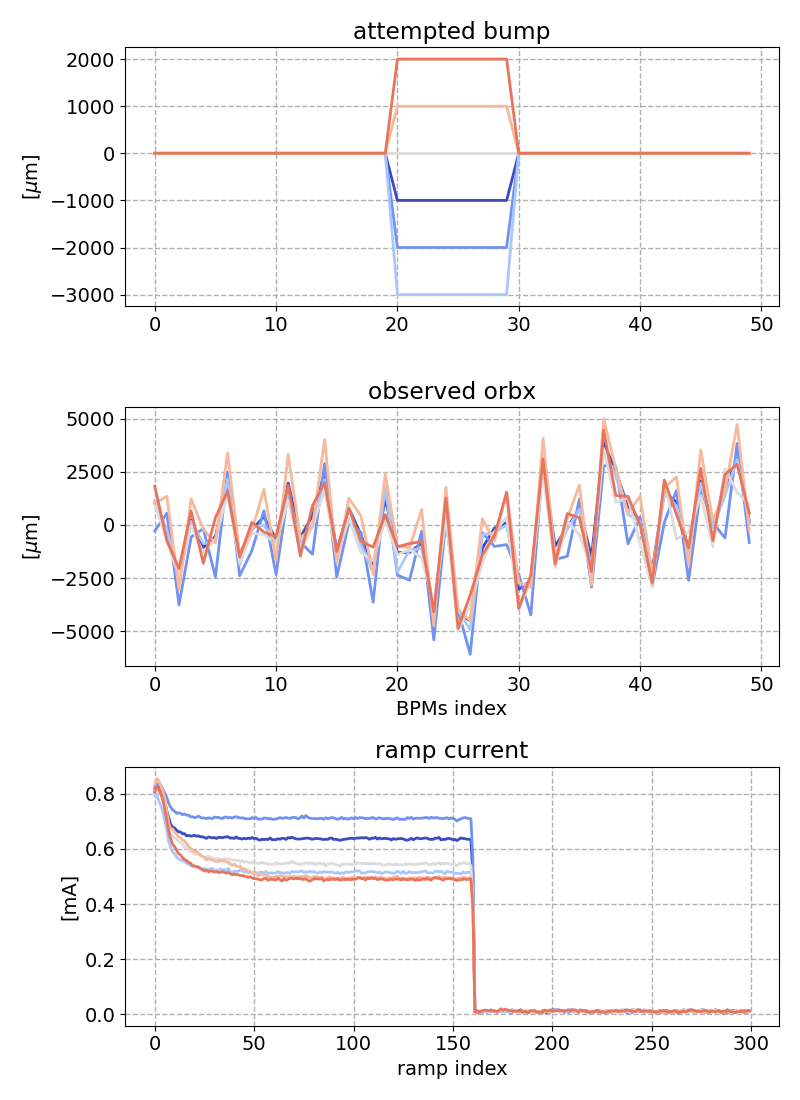
\includegraphics[height=0.9\textheight]{2024-07-12/figures/orbits_and_rampcurr_vs_bumps.png}
\end{minipage} 
\end{frame}


\begin{frame}{Bump de órbita no booster: variações de freq. RF}
\begin{minipage}{0.39\textwidth}
{\footnotesize
\begin{itemize}
    \item estudo do 2024-06-18 \href{https://cnpemcamp.sharepoint.com/:b:/s/FAC/EVB6kJl7jAZHgoUxKpIutQABaUAl3s8RLa3O1rui_7JApg?e=V9X4Yf}{\beamergotobutton{Teams FAC/Machine Studies/Files}}
    \item variações de freq. 
    \item sem efeito na eficiência a não ser p/ variações extremas
    \item investigação de efeitos de carga usando as screens da TB e BO foi abortado por problemas de controle.
\end{itemize}}
% \hsfill
\end{minipage}
\begin{minipage}{0.58\textwidth}
    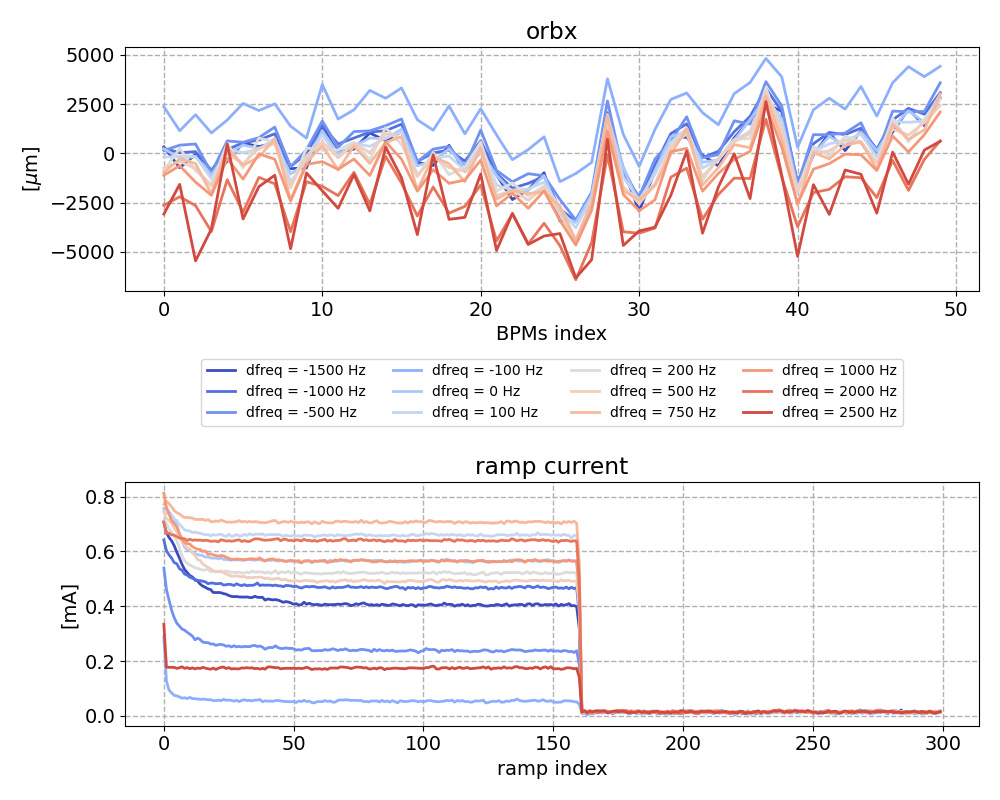
\includegraphics[width=\linewidth]{2024-07-12/figures/orbits_and_rampcurr_vs_dfreq.png}
\end{minipage} 
\end{frame}